\begin{frame}{Mapping coverage}
    \begin{columns}

        \begin{column}{0.5\textwidth}
            \textbf{Trajectory}
            $$\mathbb{X} = \underset{t \in [t_0, t_f]}{\bigcup} f_t^{-1}([0, \mathnormal{r}[)$$

            The union of all patch give the mapping coverage.
            
            \vspace{0.5cm}
            \textbf{Areas} \\
            \textit{Red area} is the set seen for sure. \\
            \textit{Orange} area is the maybe seen set. \\
            \textit{Green} area is the not seen set.
           
        \end{column}

        \begin{column}{0.5\textwidth}
            \begin{figure}
                \centering
                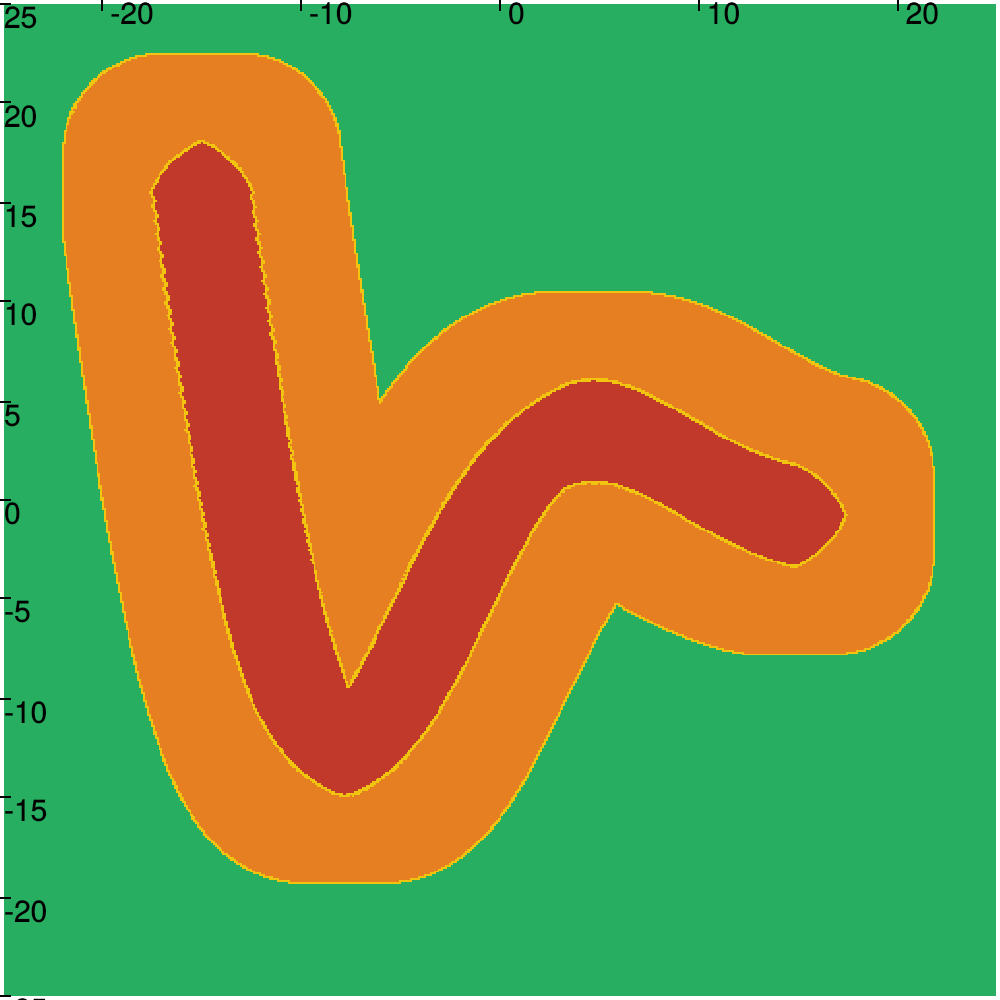
\includegraphics[width=\textwidth]{images/Thicksets/thickset_trajectory.png}
                \caption{Mapping coverage along a trajectory}
            \end{figure}
        \end{column}
    \end{columns}
\end{frame}
